\section{Diffusion Magnetic Resonance Imaging}

Diffusion magnetic resonance imaging (dMRI) is a popular MR modality that is capable of providing orientation information of brain tissue in-vivo, and thereby permitting the reconstruction and analysis of brain white matter structures with the use of computer reconstruction techniques. 

\subsection{Diffusion Weighted Image (DWI)}

The basis of dMRI is based on the observation that the location probability distribution of water molecules, which undergoes Brownian motion during diffusion, is a function of its suspension medium. The rate of diffusion can be formulated as \cite{Mukherjee2008}: 
\begin{equation}
<r^2>=6Dt
\end{equation}
where $<r^2>$ is the mean square displacement of the molecule after time $t$ with diffusion constant $D$. In an unhindered medium, such as in liquid water, its diffusion probability is can be described as an spherical volume, in other words it undergoes \textit{isotropic} diffusion. In biological tissue such as the neuron axonal bundle, its diffusion probability is then constrained to be more likely in a direction along the bundle, rather than parallel to the cross-section, its diffusion state is then described as \textit{anisotropic} (\ref{fig:diffusion}). 

\begin{figure}[ht]
\begin{center}
\begin{tabular}{c}
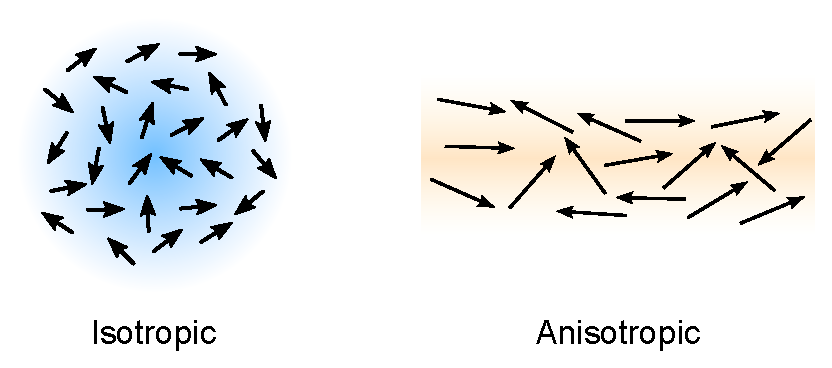
\includegraphics[width=0.8\textwidth]{diffusion.pdf}
\end{tabular}
\caption{Isotropic diffusion: diffusion of molecules have the same probable displacement in all directions. Anisotropic diffusion displacement of modules are constrained to its diffusion medium.}
\label{fig:diffusion}
\end{center}
\end{figure}

To image this difference in tissue diffusion, a diffusion-weighted imaging (DWI) pulse sequence, which is termed Stejskal-Tanner encoding, is used by adding diffusion-sensitizing gradients to a T2-weighted spin-echo sequence, before and after the 180 degrees refocusing pulse. The gradient is parameterized by the gradient amplitude $G$ in $mT/m$, duration $\delta$ in $ms$, and refocusing delay interval $\Delta$ in $ms$. 

The image contrast is determined by the amount molecular motion between the two gradients, where motion along the gradient axis results in a loss of image intensity. The contrast is defined as: 
\begin{equation}
S_i = S_0 \cdot e^{-b \cdot ADC_i}
\end{equation}
Here $S_i$ denote the image contrast at a voxel. $S_0$ the signal intensity without the gradients applied. $ADC_i$ being the apparent diffusion coefficient in the $i$ direction. $b$ is the diffusion weighted factor that is a function is the duration, strength and temporal spacing of the gradients: 
\begin{equation}
b = \gamma^2 G^2 \delta^2(\Delta - \delta/3)
\end{equation}
where $\gamma$ is the gyromagnetic ratio constant. The ADC is measured in $mm^2/s$, and denotes the average molecular diffusion area with a given acquisition time. The higher ADC values indicate higher molecular mobility. Clinical DWI sequences typically use a diffusion time of 10-50 ms, or a travel of about 10$\mu$m. Typical clinical $b$ values range from 600 to 1500, to balance signal contrast with acquisition time. 

\subsection{Diffusion Tensor Imaging}

To adequately characterize anisotropic diffusion, there must be more than one gradient directions available. In fact, it is possible to describe voxel-wise diffusion using a Gaussian diffusion model, where the diffusion anisotropy can be visualized as an ellipsoidal tensor \cite{Jones2002}. This type of imaging methodology is termed diffusion tensor imaging (DTI). At least six non-collinear gradient directions must be captured to compute the DT. In practice, up to 32 gradients directions are used clinically.

The diffusion tensor is a $3 \times 3$ symmetric matrix that describes diffusion displacement in the three major axes of diffusion: 

\begin{equation}
D=
\begin{bmatrix}
    D_{xx} & D_{xy} & D_{xz} \\
    D_{xy} & D_{yy} & D_{yz} \\
    D_{xz} & D_{yz} & D_{zz}
\end{bmatrix}
\end{equation}
Where $D_{i,j}$ is related to:

\begin{equation}
\frac{S}{S_0} = e^{-\Big(\sum\limits_{i=x,y,z} \sum\limits_{j=x,y,z} b_{i,j} \cdot D_{i,j}\Big)}
\end{equation}

and 

\begin{equation}
b_{i,j} = \gamma^2 G_i G_j \Big[ \delta^2 \Big( \Delta - \frac{\delta}{3} \Big) \Big]. 
\end{equation}

The diffusion tensor can then be diagonalized to find its eigen vectors, which are the principal axis of the diffusion ellipsoid, and from which we can obtain the eigen values (\ref{fig:tensor}): 

\begin{equation}
\Lambda = 
\begin{bmatrix}
\lambda_1 	& 0 		& 0 		\\
0 			& \lambda_2	& 0 		\\
0 			& 0 		& \lambda_3 \\
\end{bmatrix}
= R \cdot D \cdot R^T.
\end{equation}

The eigen values are measured in the same unit as ADC, which is in $mm^2/s$. Their corresponding eigen vector is denoted as $\hat{\lambda_i}$ They are ordered from the greatest to the least diffusivity magnitude. $\hat{\lambda_1}$ points to the orientation of the greatest diffusion direction, and therefore $\lambda_1$ is also referred to as "longitudinal" or "axial" diffusivity. $\hat{\lambda_2}$ and $\hat{\lambda_3}$ are the lesser orthogonal diffusion directions, and their mean magnitude gives rise to the cross-sectional, or "radial" diffusivity. 

\begin{figure}[ht]
\begin{center}
\begin{tabular}{c}
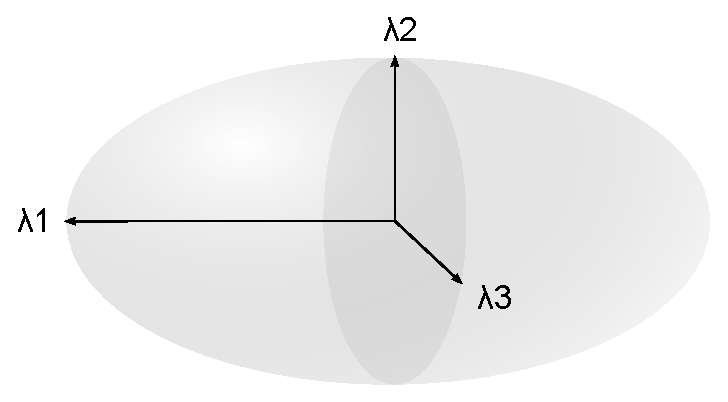
\includegraphics[width=2.5in]{tensor.pdf}
\end{tabular}
\caption{Illustration of the eigen vectors of an ellipsoid tensor.}
\label{fig:tensor}
\end{center}
\end{figure}

\subsubsection{DTI Metrics}

The Gaussian tensor eigen values form the basis of diffusivity measures that are commonly used to quantify cerebral tissue. The most common diffusivity metrics include Trace, Axial(Parallel/Primary/Longitudinal) diffusivity (AD), Radial (Perpendicular) diffusivity (RD), Mean diffusivity (MD) and fractional anisotropy, these are listed as follows: 

\begin{equation}
Trace = \sum_{i=1}^{3} \lambda_i
\end{equation}
\begin{equation}
AD = \lambda_1
\end{equation}
\begin{equation}
RD = \frac{(\lambda_2+\lambda_3)}{2}
\end{equation}
\begin{equation}
MD = \frac{\text{Trace}}{3}
\end{equation}
\begin{equation}
FA = \sqrt{\frac{3}{2}}\frac{\sqrt{(\lambda_1-MD)^2 + (\lambda_2-MD)^2 + (\lambda_3-MD)^2}}{\sqrt{\lambda_1^2+\lambda_2^2+\lambda_3^2}}
\end{equation}

FA has been found to correlate with a wide spectrum of neuromorphological changes, including but not limited to multiple sclerosis \shortcite{Cercignani2001,Ciccarelli2003d,Miron2012}, vestibular schwannomas \shortcite{Chen2011b,Taoka2006,Wai2009}, tumors \shortcite{Mori2002,Schonberg2006,Nimsky2005}, schizophrenia \shortcite{Rametti2009,Fitzsimmons2009}, traumatic brain injury \shortcite{Bendlin2008,Kinnunen2011c,Hellyer2012}. RD is found to positively correlate with degree of demyelination in multiple sclerosis \shortcite{Song2005,Song2002,Klawiter2011,Janve2013}, and well as stages of white-matter development and aging \shortcite{Counsell2006,Sala2010}, including alzheimer's disease \shortcite{Acosta-Cabronero2012}. AD is correlated positively with axonal integrity \shortcite{Song2003}, and is found to be a correlate of axonal injury \shortcite{Budde2009} such as those found in traumatic brain injury \shortcite{Kinnunen2011c} and Gulf War illness \shortcite{Rayhan2013}. MD is correlated with tissue inflammation and edema \shortcite{Senda2012g}, and is found to correlate with diffusivity changes as a result of gliomas \shortcite{Stadlbauer2007}, multiple sclerosis \shortcite{Cercignani2001,Senda2012g,DeGroot2013}, amyotrophic lateral sclerosis \shortcite{Sharma2012}, and aging \shortcite{Kantarci2011}.

\subsubsection{Limitations}

DTI is based on the Gaussian model of water diffusion, and therefore imposes an important limitation. The Gaussian tensor can derive only one diffusion direction at a given voxel, and therefore is incapable of modelling cross-fiber diffusion of two or more directions. By extension, its derived metrics (FA, AD, RD) can only characterize a single diffusion direction as well. Therefore the interpretation of these metrics in white matter that contains cross-fiber configurations is tenuous.  

\subsection{High Angular Resolution Diffusion Imaging}

In order to characterize the additional diffusion components in voxels with multiple fibres, changes in DWI acquisition strategies is necessary. A natural extension is to acquire additional diffusion directions. This type of acquisition strategies, which enable higher order diffusion modelling algorithms, are generally referred to as high angular resolution diffusion imaging (HARDI). The most wide-spread strategy is to equally distribute gradient directions as vertices of a triangle-tessellated geodesic sphere \cite{Frank2001}. Alternatively, it is also possible to distribute gradient directions in a rectilinear grid, which forms the basis of diffusion spectrum imaging (DSI) \cite{Wedeen2005}. Additional acquisition strategies such as distributing gradient directions across multiple concentric spherical shells are also actively explored \cite{Jeurissen2014a}. 

Modifications to B-value needs to be considered for HARDI. The measured diffusion contrasts are dependent on the diffusion compartment variances. Therefore higher B-values will increase the measured signals variance contrasts, and allow better separation between crossing diffusion directions. Different HARDI algorithms have different requirements on B-values. For example Q-ball imaging needs B=3000 $s/mm^2$ \cite{Descoteaux2007a}, and multi-shell acquisitions will require stepped values of B values ranging from 500  $s/mm^2 $  to greater than 3500  $s/mm^2 $ \cite{Tournier2013}. 

The determination of gradient sampling pattern and B-value directly affect acquisition time and image quality. More complex gradient sampling and higher B-values can improve tractography quality. However the acquisition time can become prohibitively long in a clinical setting. Other factors that must be considered include the nature of patient pathology, motion artifacts, and the inclusion of other imaging modalities during clinical scan sessions. 

\subsection{Spherical Deconvolution}

An end-to-end spherical deconvolution diffusion model was first proposed by Tournier et al. \cite{Tournier2004}. 
Consider a fiber population with distinct fiber components. The measured diffusion signal $S(\theta,\phi)$ can be written as:

\begin{equation}
S(\theta, \phi) = \sum_{i}^{} f_i \hat{A}_i R(\theta)
\end{equation}
where $\theta$ is the elevation angle,  $\phi$ the azimuth angle in spherical coordinates; $f_i$ is the volume fraction of the $i$-th fiber component, $\hat{A}$ is the rotation operator that orients fiber, and $R(\theta)$ is an axially symmetric response function. 

$S(\theta,\phi) $ can be rewritten as a convolution over the unit sphere of $R(\theta)$ with a fiber orientation density function (FOD) $F(\theta, \phi)$, such that:
\begin{equation}
S(\theta, \phi) = F(\theta, \phi) \otimes R(\theta)
\end{equation}

With this approach, the FOD can be estimated using the reverse spherical deconvolution, using spherical and rotational harmonics \cite{Healy1998}. Spherical harmonics are orthonormal basis functions over a sphere, and therefore can approximate any symmetric diffusion geometry in the spherical q-space. The rotational harmonics similarly form the orthonormal basis over all possible rotations, and can represent any symmetric fiber configurations. The harmonics have two important parameters: the harmonic order $l$ and phase factor $m$, with $ -l \leq m \leq l $ for each harmonic order level $l$. The odd $l$ harmonics represent antisymmetric functions, while the even $l$ harmonics represent symmetric functions (\ref{fig:harmonics}). 

\begin{figure}[ht]
\begin{center}
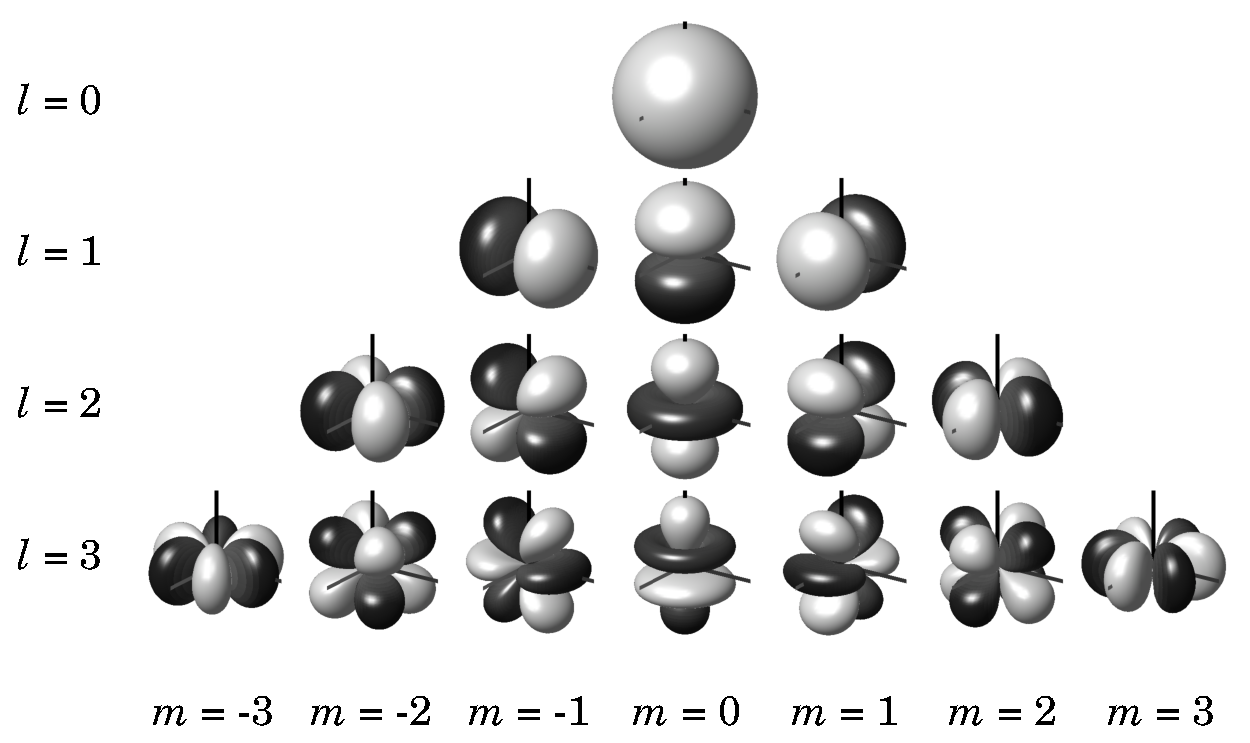
\includegraphics[width=\textwidth]{harmonics.pdf}
\caption{Visualization of the spherical harmonic functions up to l=3. Modified from \protect\cite{sh-image-wikipedia}}
\label{fig:harmonics}
\end{center}
\end{figure}

Spherical decovolution is considered to be the action of a set of rotations on a function over a sphere. Given $F^l $ as a vector of $l$th order spherical harmonic decomposition of  $F(\theta,\phi)$, with vector length $(2l + 1)$, and $R^l$ as the $l$th order rotational harmonic decomposite of $R(\theta)$, with vector length $(2l+1)^2$. The spherical harmonic representation of $S(\theta,\phi)$ is then:

\begin{equation}
S^l = R^l F^l
\end{equation}

To reduce the number of parameters to be computed, we can make the further assumption that the diffusion process is symmetric, and therefore the odd $l$ harmonic orders can be ignored, with only the even harmonics considered. 
The response function $R(\theta)$ can be directly estimated from the dataset by supplying DWI region with high anisotropy from a single fiber bundle, such as the body of the corpus callosum. 

The maximum harmonic order $l_max$ that can be estimated is dependent on the obtained number of directions. For example, $l_max$ = 8 requires 45 directions, $l_max$ = 10 requires 66 directions, and so on. Larger $l_max$ are more sensitive to noise, which is a weakness for the first spherical deconvolution algorithm \cite{Tournier2004}. 

\subsubsection{Constrained Spherical Deconvolution}
Further advances to the estimation method of the spherical deconvolution model made it more robust to noise \cite{Tournier2007b}. The noise of SD estimation is represented as spurious negative lobes in FOD, which are physically impossible, and do not represent any real phenomenon. To mitigate this, a non-negativity constraint is added. This method is referred to as \textit{constrained spherical deconvolution} (CSD). 

The CSD constraint is applied iteratively using Tikhonov regularization \cite{Hansen1998}. The procedure involves obtaining an initial FOD estimate, and a set of directional peaks are then identified. The Tikhonov regularization then constraints the negative peaks to zero, and a new set of FOD and peaks are obtained. The process is applied iteratively until convergence, and the final constrained FOD is obtained. 

The Tikhonov regularization minimizes the weighted sum with two terms:
\begin{equation}
\|{Af - b}^2\|^2 + \lambda^2 \| l(f - f')\|^2
\end{equation}
Where the first term is a linear least-square fit of solution $f$ to to data $b$ with problem matrix $A$. 
In terms of CSD, $f$ corresponds to the SH coefficients of the FOD, $b$ is the measured signal and $A$ is:
\begin{equation}
A = QR
\end{equation}
Where $Q$ is the SH coefficient to DW intensity mapping, and $R$ is the spherical deconvolution. 
The regularization term is the constrained matrix $L$ multiplying the norm of $f$ relative to an initial estimate $f'$. The parameter $\lambda$ controls the regularization amount, with $\lambda=0$ having no regularization, to $\lambda\rightarrow \infty $ making the solution tend to $f'$. 

In CSD, the $f'=0$ and $L$ maps $f$ to orientations that have zero amplitude. During initiation, $f_0$ is estimated using spherical deconvolution with a low-pass filter \cite{Tournier2004}, and truncated to $l_max = 4$. The FOD amplitudes $u$ are then computed along N uniformly distributed directions (By default, MRTrix uses $N=300$) where
\begin{equation}
u = P f_i
\end{equation}
L is then formed as:
\begin{equation}
L_{m,n} = 
	\begin{cases}
		P_{m,n}, & u_m < \tau \\
		0 &	u_m \geq \tau 
	\end{cases}
\end{equation}
where $\tau$ is the amplitude threshold. In practice $\tau$ is set to 10\% of mean FOD amplitude. 
The improved iterative $f_i$ is then solved by incorporating the new FOD amplitude information by:
\begin{equation}
f_{i+1} = \text{argmin}\{ \|Af_i - b\|^2 + \lambda^2 \|L f_i\|^2  \}
\end{equation}
The FOD estimate becomes stable when matrix L converges, which take about 10 iterations. 

CSD is robust to noise at relatively low B-values, and is capable of good quality FOD estimates at $B=1000 s/mm^2$. This means that existing DTI protocols can be extended for high order HARDI tractography by simply increasing the number of directions. With CSD, a 60 direction DWI acquisition can be used to confidently derive FOD with $l_{max}=8 $, and up to $l_{max}=12$ with super resolution enabled \cite{Tournier2007b} (Figure \ref{fig:csd}). 

\begin{figure}[ht]
\begin{center}
\begin{tabular}{c}
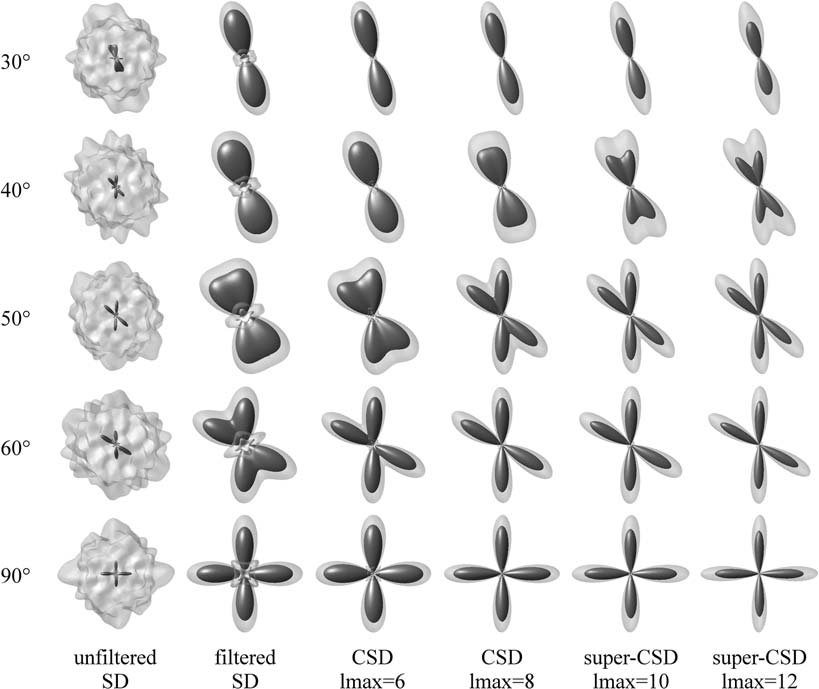
\includegraphics[width=\textwidth]{csd-angles}
\end{tabular}
\caption{ Comparison of angle discrimination ability and CSD FOD. B-value=3000 \protect $s/mm^2$. Taken from \protect \cite{Tournier2007b} } 
\label{fig:csd}
\end{center}
\end{figure}

\subsection{Tractography}
Tractography is defined as the construction, or propagation of streamline from an underlying field of orientation information, in order to visualize continuous structures within a volume.  The orientation field is generally provided as a 3D matrix of directional information obtained from DTI, CSD, or other methods. For example, in DTI the directions are the eigen vector with the greatest magnitude $\hat{\lambda_1}$; for CSD, the directional vectors would be peaks from the FOD. 

Applying pathway tracking to DWI imaging was first explored by Mori \cite{Mori2002b} and Basser\cite{Basser2000}. The family of methods that propagates by deterministic algorithms based on local orientation data is collectively called deterministic tractography. The first tracking algorithms were applied to DTI using step-wise polyline propagators that followed local DT tensors \cite{Conturo1999}. Further refinement of the line propagator to include neighbouring DT tensors, and interpolation of the local DT directions in order to obtain a smooth curve \cite{Mori2002b}. Basser introduced Runge-Kutta integration to allow more robust path-tracing when faced with noise in the local directions \cite{Basser2000}. Another similar path-integral method was also proposed by Tuch \cite{Tuch2000d}. The integrated tractography approaches are now standard practice for deterministic tractography \cite{Tournier2004,Pieper2004}. 

Deterministic tractography lends itself naturally to anatomical interpretation and further geometric analysis. It was traditionally paired with DTI, and so was thought to be limited in the case of crossing fibers. Other methods attempted to circumvent the limitation with probabilistic approaches that include white matter tissue priors in the fiber propagation model. The most popular of the probabilistic approach is the FSL software's probabilistic tractography module (FDT) \cite{Behrens2007}, which also includes a model-based ball-and-stick diffusion model that can resolve 2-fiber crossings. The FDT software produces visitation images of its probabilistic streams that collate the probability of tract propagation at each voxel.  The visitation image, however, is hard to interpret and localize, and therefore does not rival deterministic methods in surgical visualization.

The availability of higher order HARDI methods, especially in CSD allows the reinterpretation of FOD as local fiber orientation probability distribution \cite{Tournier2010,Jeurissen2011b}. Development of a probabilistic streamline propagator based on CSD can now combine the advantage of probabilistic models with the geometric interpretability of deterministic tractography. 

\subsubsection{Applications}
Tractography permits the mapping of white matter structures with computer graphic and statistic methods. It permits the study of brain structural connectivity at individual level \cite{Boorman2007} and group level \cite{Meskaldji2013},  circuitry mapping \cite{Kirsch2015} and macro-structural insights between the brain hemispheres \cite{Kucyi2012a}. It is often paired with functional connectivity for studies in multiple sclerosis \cite{Zhong2016,Rocca2007a,Kucyi2015}, chronic pain \cite{Mansour2013,Seifert2011,Wiech2014}, and other areas of study such as empathy \cite{Bernhardt2014}, and aphasia \cite{Catani2013c}.

Tractography is also capable of fine-grained neuroanatomy visualizations \cite{Hodaie2010, Chen2015c}, and therefore is important in the advancement of surgical visualization \cite{Chen2011b,Rosen2015,Hodaie2012g,Taoka2006,Sherbondy2008,Muthusamy2007} and planning \cite{Golby2011}. 

\begin{figure}[ht]
\begin{center}
\begin{tabular}{c}
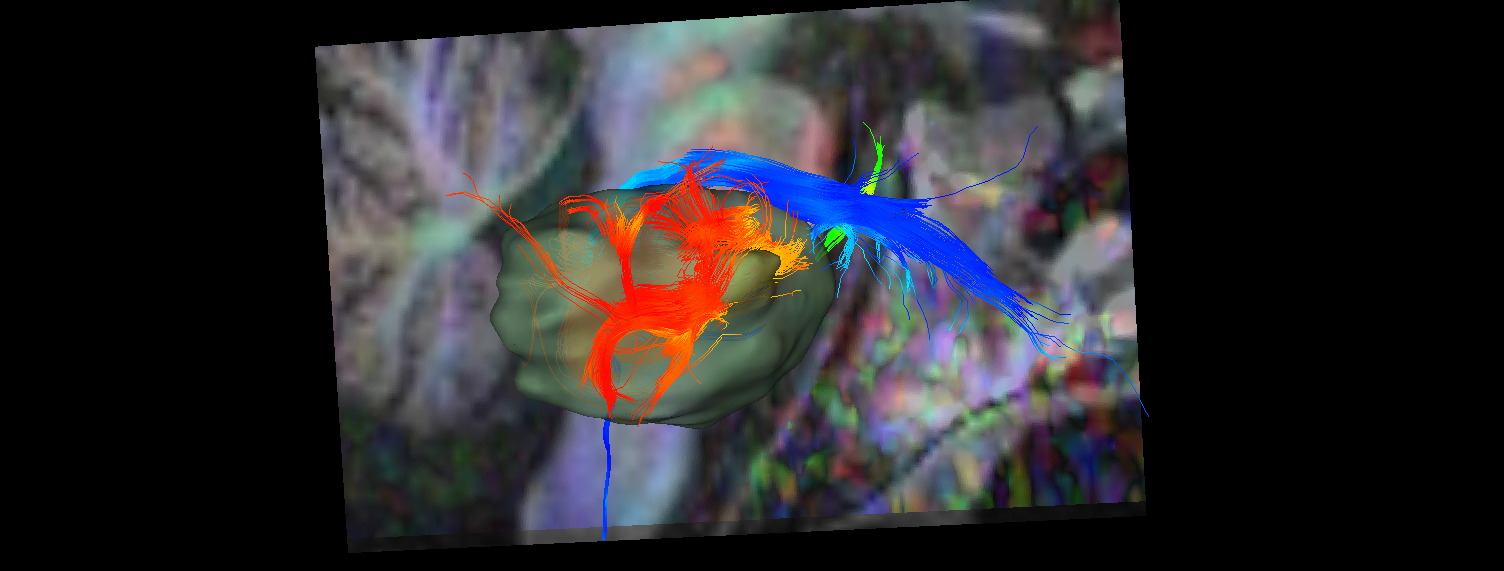
\includegraphics[width=\textwidth]{tractography1}
\end{tabular}
\caption{Example of cranial nerve reconstruction with deterministic tractography.} 
\label{fig:tract1}
\end{center}
\end{figure}

